% Created 2023-11-21 Tue 00:25
% Intended LaTeX compiler: pdflatex
\documentclass[11pt]{article}
\usepackage[utf8]{inputenc}
\usepackage[T1]{fontenc}
\usepackage{graphicx}
\usepackage{longtable}
\usepackage{wrapfig}
\usepackage{rotating}
\usepackage[normalem]{ulem}
\usepackage{amsmath}
\usepackage{amssymb}
\usepackage{capt-of}
\usepackage{hyperref}
\usepackage{siunitx}
\author{Hankertrix}
\date{\today}
\title{Physics Inductors Cheat Sheet}
\hypersetup{
 pdfauthor={Hankertrix},
 pdftitle={Physics Inductors Cheat Sheet},
 pdfkeywords={},
 pdfsubject={},
 pdfcreator={Emacs 29.1 (Org mode 9.6.6)}, 
 pdflang={English}}
\begin{document}

\maketitle
\setcounter{tocdepth}{2}
\tableofcontents \clearpage
\section{Definitions}
\label{sec:org4b5990b}

\subsection{Potential difference across an inductor}
\label{sec:org4df372e}
The potential difference across an inductor depends on the \textbf{rate of change of the current}.
\[V_{ab} = L \frac{dI}{dt}\]

Where:
\begin{itemize}
\item \(V_{ab}\) is the potential difference across the conductor.
\item \(L\) is the self inductance of the conductor.
\item \(\frac{dI}{dt}\) is the rate of change of the current with respect to time.
\end{itemize}

\subsection{Inductive reactance (SI Unit: \(\unit{\ohm}\))}
\label{sec:org438c068}
\[X_L = \omega L = 2 \pi f L\]

Where:
\begin{itemize}
\item \(X_L\) is the inductive reactance.
\item \(\omega\) is the angular frequency.
\item \(L\) is the inductance.
\item \(f\) is the frequency.
\end{itemize}

\subsection{Capacitive reactance (SI Unit: \(\unit{\ohm}\))}
\label{sec:org35f6663}
\[X_C = \frac{1}{\omega C} = \frac{1}{2 \pi f C}\]

Where:
\begin{itemize}
\item \(X_C\) is the capacitive reactance.
\item \(\omega\) is the angular frequency.
\item \(C\) is the capacitance.
\item \(f\) is the frequency.
\end{itemize}

\subsection{Resonance in A.C. circuits}
\label{sec:org5219c14}
\[f_0 = \frac{\omega_0}{2 \pi} = \frac{1}{2 \pi} \sqrt{\frac{1}{LC}}\]

Where:
\begin{itemize}
\item \(f_0\) is the resonance frequency.
\item \(\omega_0\) is the angular frequency.
\item \(L\) is the impedance of the circuit.
\item \(C\) is the capacitance of the circuit.
\end{itemize}


\section{RL circuit}
\label{sec:org1bbabe5}
\begin{center}
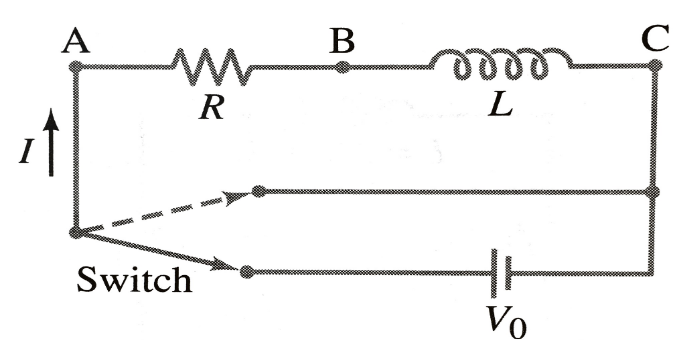
\includegraphics[width=.9\linewidth]{./images/rl-circuit.png}
\end{center}

Consider the circuit shown above. At the instant the switch is closed, current starts to flow. The voltage or e.m.f induced across the inductor by this change in current from zero to some finite value opposes the change that induces it.
\\[0pt]

Derivation of \(I(t)\). By Kirchhoff's voltage rule:
\begin{align*}
V_0 - IR - L \frac{dI}{dt} = 0 \\
L \frac{dI}{dt} &= V_0 - IR \\
\int_0^I \frac{dI}{V_0 - IR} &= \int_0^t \frac{dt}{L} \\
-\frac{1}{R} \left[\ln |V_0 - IR| \right]_0^I &= \frac{1}{L}[t]_0^t \\
-\frac{1}{R} \left(\ln |V_0 - IR| - \ln |V_0| \right) &= \frac{t}{L} \\
\ln |V_0 - IR| - \ln |V_0| &= -\frac{Rt}{L} \\
\ln \left| \frac{V_0 - IR}{V_0} \right| &= -\frac{Rt}{L} \\
\frac{V_0 - IR}{V_0} &= e^{-\frac{Rt}{L}} \\
V_0 - IR &= V_0 e^{-\frac{Rt}{L}} \\
IR &= V_0 - V_0 e^{- \frac{Rt}{L}} \\
I(t) &= \frac{V_0}{R} \left(1 - e^{- \frac{Rt}{L}} \right)
\end{align*}

\subsection{Application: surge arrestor}
\label{sec:org00ac006}
\begin{itemize}
\item If lightning strikes part of an electrical power transmission system, it causes a sudden spike in voltage that can damage the components of the system.
\item To minimise these effects, large inductors are incorporated into the transmission system.
\item These use the principle that an inductor opposes and suppresses any rapid changes in the current.
\end{itemize}


\section{LC circuit (without voltage source)}
\label{sec:org5011e10}

\begin{center}
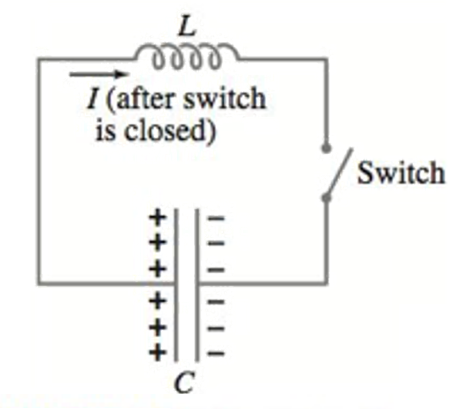
\includegraphics[scale=0.8]{./images/lc-circuit.png}
\end{center}

By Kirchhoff's voltage law:
\[-L \frac{dI}{dt} + \frac{Q}{C} = 0 \tag{1}\]

The current comes from the decrease of the capacitor's charge:
\[I = - \frac{dQ}{dt} \tag{2}\]

Substituting \((2)\) into \((1)\):
\[- L \cdot -\frac{d^2Q}{dt^2} + \frac{Q}{C} = 0\]
\[\frac{d^2Q}{dt^2} + \frac{Q}{LC} = 0 \tag{3}\]

Trying \(Q = Q_0 \cos (\omega t + \phi)\) with \((3)\):
\[- \omega^2 Q_0 \cos (\omega t + \phi) + \frac{1}{LC} Q_0 \cos (\omega t + \phi) = 0\]
\[\left(- \omega^2 + \frac{1}{LC} \right) \cos ( \omega t + \phi ) = 0\]
\[\Longrightarrow = \left(- \omega^2 + \frac{1}{LC} \right) = 0\]
\[\omega = 2 \pi f = \sqrt{\frac{1}{LC}}\]

\subsection{Graph}
\label{sec:org4b6fad2}

\begin{center}
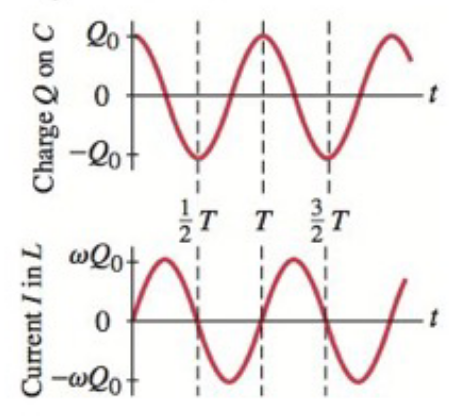
\includegraphics[scale=0.8]{./images/lc-circuit-graph.png}
\end{center}

\subsection{Total energy in the circuit}
\label{sec:org9b8bcea}
The total energy in the circuit is constant, it oscillates between the capacitor and the inductor.

\begin{align*}
U &= U_E + U_B \\
&= \frac{1}{2} \frac{Q^2}{C} + \frac{1}{2} LI^2 \\
&= \frac{Q_0}{2C} \left[\cos^2 (\omega t + \phi) + \sin^2 (\omega t + \phi) \right] \\
&= \frac{Q_0^2}{2C}
\end{align*}

The frequency of energy oscillations is twice that of the frequency of charge and current oscillations.

\begin{center}
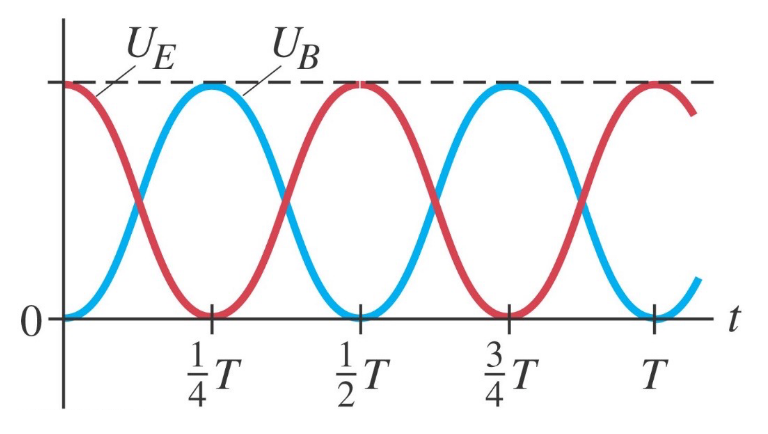
\includegraphics[scale=0.6]{./images/lc-circuit-energy.png}
\end{center}


\section{RCL circuit (without voltage source)}
\label{sec:orgb82d42f}

\begin{center}
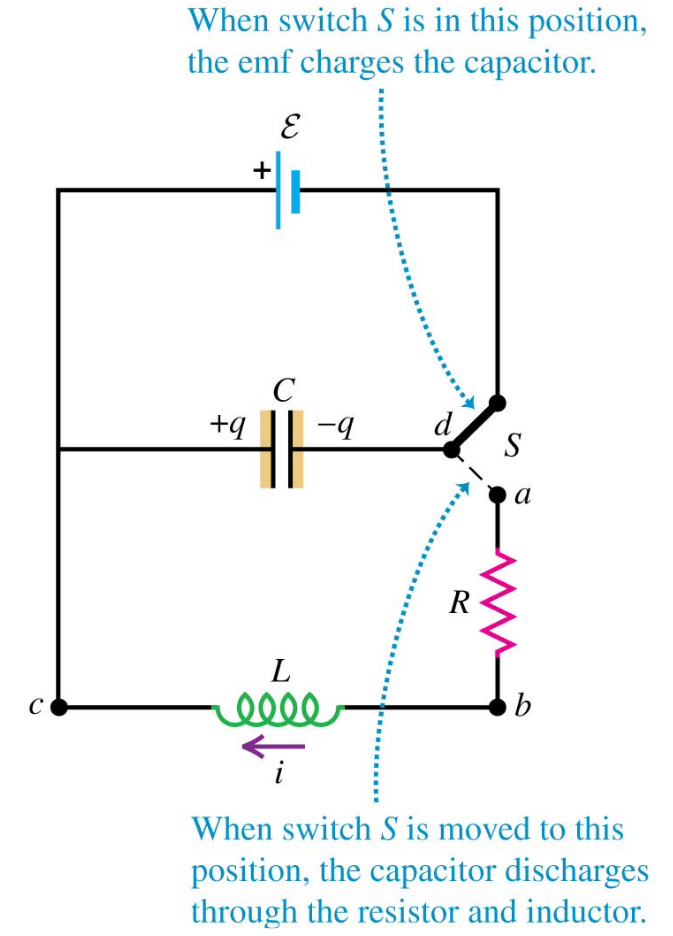
\includegraphics[scale=0.52]{./images/rcl-circuit.png}
\end{center}

Consider the circuit above. The e.m.f source charges the capacitor initially. When the switch is moved to the lower position, we have an inductor with inductance \(L\) and a resistor of resistance \(R\) connected in series across the terminals of a charged capacitor, forming an \textbf{RCL series circuit}. An RCL circuit exhibits damped harmonic motion if the resistance is not too large.
\\[0pt]

The charge as a function of time is a sinusoidal oscillation with an exponentially decaying amplitude, and angular frequency:

\[\omega ' = \sqrt{\frac{1}{LC} - \frac{R^2}{4L^2}}\]

Where:
\begin{itemize}
\item \(\omega '\) is the angular frequency of under damped oscillations in an L-R-C series circuit.
\item \(L\) is the inductance of the circuit.
\item \(C\) is the capacitance of the circuit.
\item \(R\) is the resistance of the circuit.
\end{itemize}


\section{RCL circuit}
\label{sec:orgec043c1}
\begin{center}
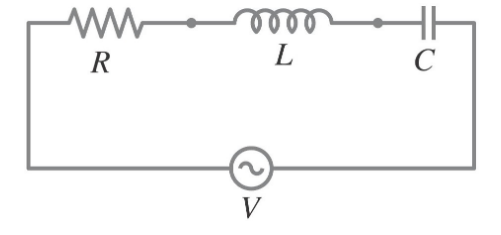
\includegraphics[width=.9\linewidth]{./images/rcl-circuit-with-source.png}
\end{center}

\subsection{Phasor diagram analysis}
\label{sec:org19ffac3}
\begin{center}
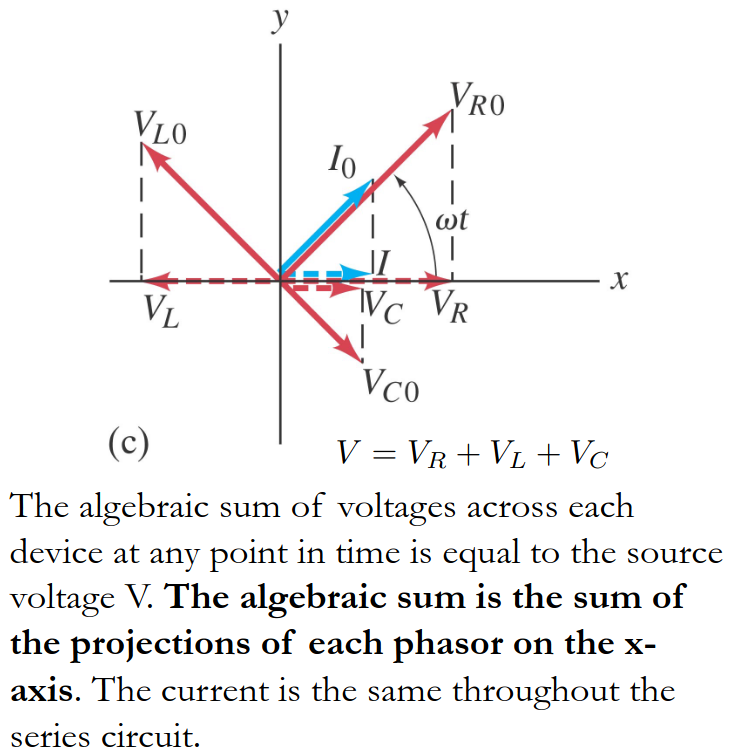
\includegraphics[width=.9\linewidth]{./images/rcl-circuit-phasor-diagram.png}
\end{center}

\subsection{Impedance}
\label{sec:org3aad5c1}
\[Z = \sqrt{R^2 + \left(\omega L - \frac{1}{\omega C} \right)^2}\]

Where:
\begin{itemize}
\item \(Z\) is the impedance of the circuit.
\item \(R\) is the resistance of the circuit.
\item \(\omega\) is the angular frequency.
\item \(L\) is the inductance of the circuit.
\item \(C\) is the capacitance of the circuit.
\end{itemize}

\subsection{Current}
\label{sec:org76fbd0e}
\[I(t) = I_0 \cos \omega t\]

\begin{itemize}
\item \(I(t)\) is the current.
\item \(I_0\) is the peak current.
\item \(\omega\) is the angular frequency.
\item \(t\) is the time.
\end{itemize}

\subsection{Voltage}
\label{sec:org013a523}
\[V(t) = I_0 Z \cos (\omega t + \phi)\]

\begin{itemize}
\item \(V(t)\) is the voltage
\item \(I_0\) is the peak current.
\item \(Z\) is the impedance.
\item \(\omega\) is the angular frequency.
\item \(t\) is the time.
\item \(\phi\) is the phase angle between the voltage and the current.
\end{itemize}

\newpage

\subsection{Phase angle between the voltage and the current}
\label{sec:org8f3d702}
\begin{center}
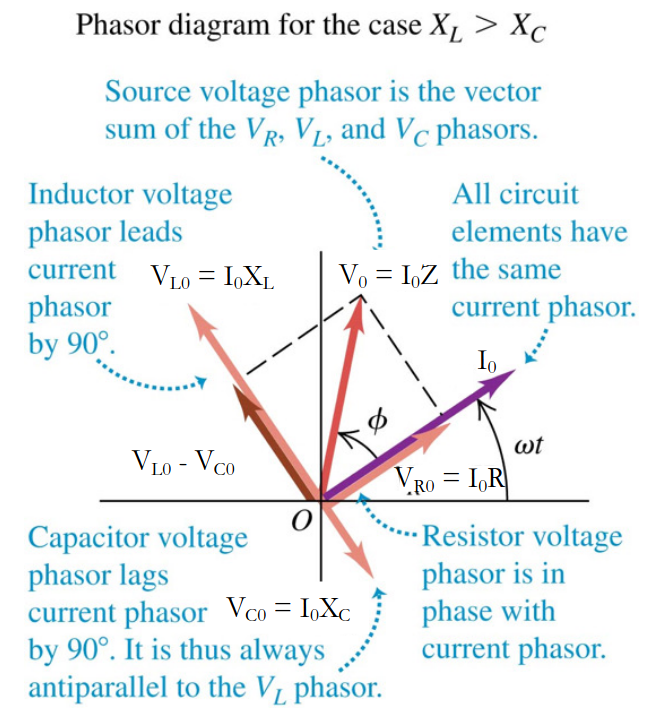
\includegraphics[width=.9\linewidth]{./images/rcl-circuit-phasor-diagram-phase-angle.png}
\end{center}

\[\phi = \arctan \left(\frac{X_L - X_C}{R} \right)\]

Where:
\begin{itemize}
\item \(\phi\) is the phase angle between the voltage and the current.
\item \(X_L\) is the inductive reactance.
\item \(X_C\) is the capacitive reactance.
\item \(R\) is the resistance of the circuit.
\end{itemize}



\section{A.C. circuit components}
\label{sec:orga952f94}

\subsection{Resistor}
\label{sec:org336aec6}

\subsubsection{Current}
\label{sec:orgf3fe8f7}
The current through a resistor is \textbf{in phase} with the voltage. The root-mean-square current is an average measure of the current.
\[I_{rms} = \frac{I_0}{\sqrt{2}}\]

Where:
\begin{itemize}
\item \(I_{rms}\) is the root-mean-square current.
\item \(I_0\) is the peak current.
\end{itemize}

\subsection{Inductor}
\label{sec:org9e60949}

\subsubsection{Voltage}
\label{sec:orgc2f8110}
The voltage across an inductor is given by:
\begin{align*}
V &= L\frac{dI}{dt} \\
&= - \omega L I_0 \sin \omega t \\
&= \omega L I_0 \cos \left(\omega t + \frac{\pi}{2} \right) \\
&= V_0 \cos \left(\omega t + \frac{\pi}{2} \right)
\end{align*}

Where:
\begin{itemize}
\item \(L\) is the inductance of the inductor.
\item \(\frac{dI}{dt}\) is the rate of change of current.
\item \(V\) is the voltage.
\item \(I_0\) is the peak current.
\item \(\omega\) is the angular frequency.
\item \(t\) is the time.
\item \(V_0\) is the peak voltage.
\end{itemize}

\subsubsection{Current}
\label{sec:orge4d6b3e}
The current through an inductor \textbf{lags} the voltage by \(90^{\circ}\).
\[I_0 = \frac{V_0}{\omega L}\]

Where:
\begin{itemize}
\item \(I_0\) is the peak current.
\item \(V_0\) is the peak voltage.
\item \(\omega\) is the angular frequency.
\item \(L\) is the inductance of the inductor.
\end{itemize}

\subsection{Capacitor}
\label{sec:orge20c5ff}

\subsubsection{Voltage}
\label{sec:orgacdcdfa}
The voltage across a capacitor is given by:
\begin{align*}
V &= \frac{Q}{C} \\
&= \frac{1}{C} \int I_0 \cos \omega t \, dt \\
&= \frac{I_0}{\omega C} \sin \omega t \\
&= \frac{I_0}{\omega C} \cos \left(\omega t - \frac{\pi}{2} \right) \\
&= V_0 \cos \left( \omega t - \frac{\pi}{2} \right)
\end{align*}

Where:
\begin{itemize}
\item \(V\) is the voltage.
\item \(Q\) is the charge held in the capacitor.
\item \(C\) is the capacitance of the capacitor.
\item \(I_0\) is the peak current.
\item \(\omega\) is the angular frequency.
\item \(t\) is the time.
\item \(V_0\) is the peak voltage.
\end{itemize}

\subsubsection{Current}
\label{sec:org082cb14}
The current through a capacitor \textbf{leads} the voltage by \(90^{\circ}\).
\[I_0 = V_0 \omega C\]

Where:
\begin{itemize}
\item \(I_0\) is the peak current.
\item \(V_0\) is the peak voltage.
\item \(\omega\) is the angular frequency.
\item \(C\) is the capacitance of the capacitor.
\end{itemize}


\subsection{High pass filter}
\label{sec:org025e516}
A high pass filter is a filter that filters out low frequencies. Think of the name as high frequencies passing through the filter unhindered.

\begin{center}
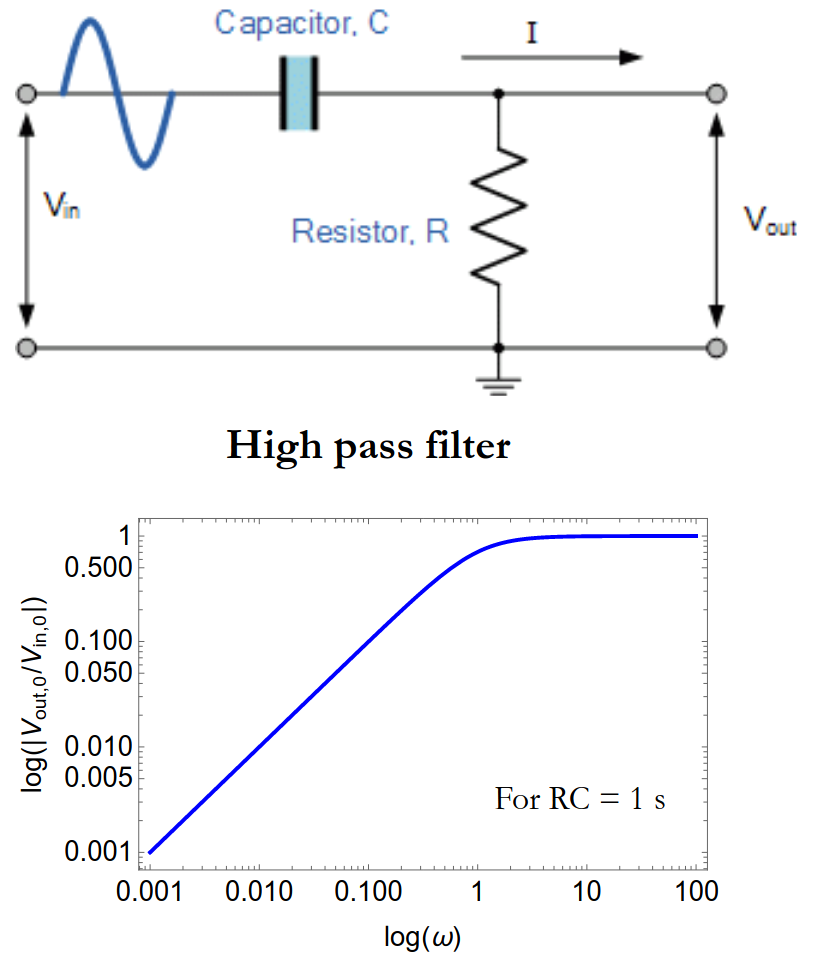
\includegraphics[scale=0.69]{./images/high-pass-filter.png}
\end{center}

\subsection{Low pass filter}
\label{sec:org0be4151}
A low pass filter is a filter that filters out high frequencies. Think of the name as low frequencies passing through the filter unhindered.

\begin{center}
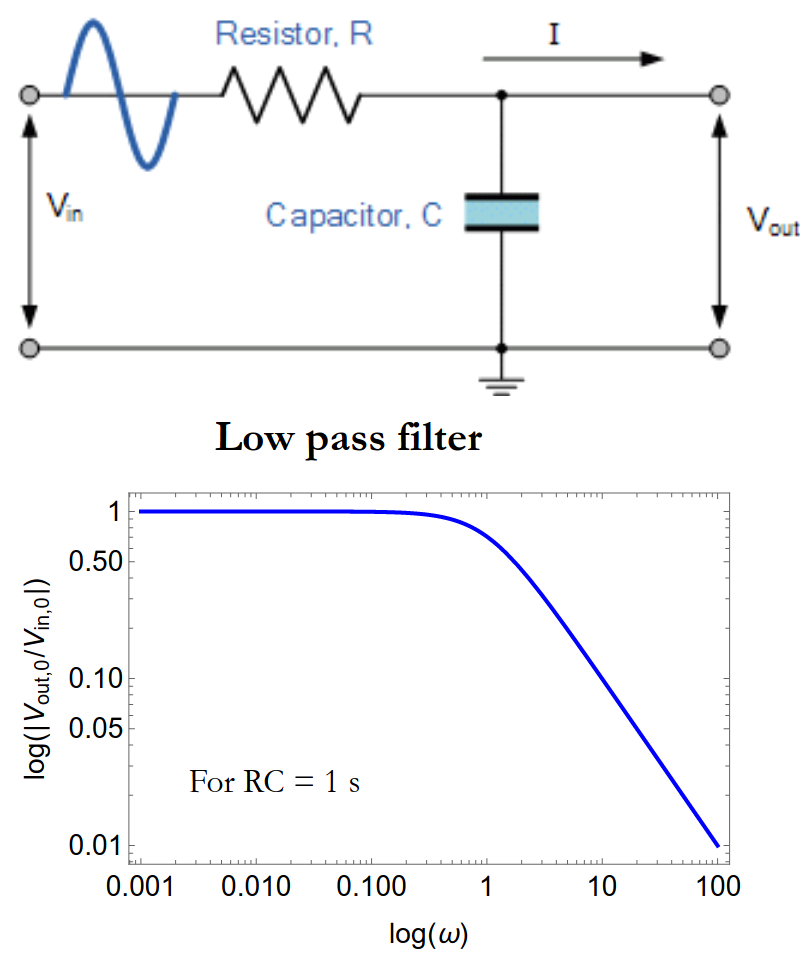
\includegraphics[width=.9\linewidth]{./images/low-pass-filter.png}
\end{center}
\end{document}